\documentclass[]{article}
\usepackage{lmodern}
\usepackage{amssymb,amsmath}
\usepackage{ifxetex,ifluatex}
\usepackage{fixltx2e} % provides \textsubscript
\ifnum 0\ifxetex 1\fi\ifluatex 1\fi=0 % if pdftex
  \usepackage[T1]{fontenc}
  \usepackage[utf8]{inputenc}
\else % if luatex or xelatex
  \ifxetex
    \usepackage{mathspec}
  \else
    \usepackage{fontspec}
  \fi
  \defaultfontfeatures{Ligatures=TeX,Scale=MatchLowercase}
\fi
% use upquote if available, for straight quotes in verbatim environments
\IfFileExists{upquote.sty}{\usepackage{upquote}}{}
% use microtype if available
\IfFileExists{microtype.sty}{%
\usepackage{microtype}
\UseMicrotypeSet[protrusion]{basicmath} % disable protrusion for tt fonts
}{}
\usepackage[margin=1in]{geometry}
\usepackage{hyperref}
\hypersetup{unicode=true,
            pdfborder={0 0 0},
            breaklinks=true}
\urlstyle{same}  % don't use monospace font for urls
\usepackage{color}
\usepackage{fancyvrb}
\newcommand{\VerbBar}{|}
\newcommand{\VERB}{\Verb[commandchars=\\\{\}]}
\DefineVerbatimEnvironment{Highlighting}{Verbatim}{commandchars=\\\{\}}
% Add ',fontsize=\small' for more characters per line
\usepackage{framed}
\definecolor{shadecolor}{RGB}{248,248,248}
\newenvironment{Shaded}{\begin{snugshade}}{\end{snugshade}}
\newcommand{\KeywordTok}[1]{\textcolor[rgb]{0.13,0.29,0.53}{\textbf{#1}}}
\newcommand{\DataTypeTok}[1]{\textcolor[rgb]{0.13,0.29,0.53}{#1}}
\newcommand{\DecValTok}[1]{\textcolor[rgb]{0.00,0.00,0.81}{#1}}
\newcommand{\BaseNTok}[1]{\textcolor[rgb]{0.00,0.00,0.81}{#1}}
\newcommand{\FloatTok}[1]{\textcolor[rgb]{0.00,0.00,0.81}{#1}}
\newcommand{\ConstantTok}[1]{\textcolor[rgb]{0.00,0.00,0.00}{#1}}
\newcommand{\CharTok}[1]{\textcolor[rgb]{0.31,0.60,0.02}{#1}}
\newcommand{\SpecialCharTok}[1]{\textcolor[rgb]{0.00,0.00,0.00}{#1}}
\newcommand{\StringTok}[1]{\textcolor[rgb]{0.31,0.60,0.02}{#1}}
\newcommand{\VerbatimStringTok}[1]{\textcolor[rgb]{0.31,0.60,0.02}{#1}}
\newcommand{\SpecialStringTok}[1]{\textcolor[rgb]{0.31,0.60,0.02}{#1}}
\newcommand{\ImportTok}[1]{#1}
\newcommand{\CommentTok}[1]{\textcolor[rgb]{0.56,0.35,0.01}{\textit{#1}}}
\newcommand{\DocumentationTok}[1]{\textcolor[rgb]{0.56,0.35,0.01}{\textbf{\textit{#1}}}}
\newcommand{\AnnotationTok}[1]{\textcolor[rgb]{0.56,0.35,0.01}{\textbf{\textit{#1}}}}
\newcommand{\CommentVarTok}[1]{\textcolor[rgb]{0.56,0.35,0.01}{\textbf{\textit{#1}}}}
\newcommand{\OtherTok}[1]{\textcolor[rgb]{0.56,0.35,0.01}{#1}}
\newcommand{\FunctionTok}[1]{\textcolor[rgb]{0.00,0.00,0.00}{#1}}
\newcommand{\VariableTok}[1]{\textcolor[rgb]{0.00,0.00,0.00}{#1}}
\newcommand{\ControlFlowTok}[1]{\textcolor[rgb]{0.13,0.29,0.53}{\textbf{#1}}}
\newcommand{\OperatorTok}[1]{\textcolor[rgb]{0.81,0.36,0.00}{\textbf{#1}}}
\newcommand{\BuiltInTok}[1]{#1}
\newcommand{\ExtensionTok}[1]{#1}
\newcommand{\PreprocessorTok}[1]{\textcolor[rgb]{0.56,0.35,0.01}{\textit{#1}}}
\newcommand{\AttributeTok}[1]{\textcolor[rgb]{0.77,0.63,0.00}{#1}}
\newcommand{\RegionMarkerTok}[1]{#1}
\newcommand{\InformationTok}[1]{\textcolor[rgb]{0.56,0.35,0.01}{\textbf{\textit{#1}}}}
\newcommand{\WarningTok}[1]{\textcolor[rgb]{0.56,0.35,0.01}{\textbf{\textit{#1}}}}
\newcommand{\AlertTok}[1]{\textcolor[rgb]{0.94,0.16,0.16}{#1}}
\newcommand{\ErrorTok}[1]{\textcolor[rgb]{0.64,0.00,0.00}{\textbf{#1}}}
\newcommand{\NormalTok}[1]{#1}
\usepackage{graphicx,grffile}
\makeatletter
\def\maxwidth{\ifdim\Gin@nat@width>\linewidth\linewidth\else\Gin@nat@width\fi}
\def\maxheight{\ifdim\Gin@nat@height>\textheight\textheight\else\Gin@nat@height\fi}
\makeatother
% Scale images if necessary, so that they will not overflow the page
% margins by default, and it is still possible to overwrite the defaults
% using explicit options in \includegraphics[width, height, ...]{}
\setkeys{Gin}{width=\maxwidth,height=\maxheight,keepaspectratio}
\IfFileExists{parskip.sty}{%
\usepackage{parskip}
}{% else
\setlength{\parindent}{0pt}
\setlength{\parskip}{6pt plus 2pt minus 1pt}
}
\setlength{\emergencystretch}{3em}  % prevent overfull lines
\providecommand{\tightlist}{%
  \setlength{\itemsep}{0pt}\setlength{\parskip}{0pt}}
\setcounter{secnumdepth}{0}
% Redefines (sub)paragraphs to behave more like sections
\ifx\paragraph\undefined\else
\let\oldparagraph\paragraph
\renewcommand{\paragraph}[1]{\oldparagraph{#1}\mbox{}}
\fi
\ifx\subparagraph\undefined\else
\let\oldsubparagraph\subparagraph
\renewcommand{\subparagraph}[1]{\oldsubparagraph{#1}\mbox{}}
\fi

%%% Use protect on footnotes to avoid problems with footnotes in titles
\let\rmarkdownfootnote\footnote%
\def\footnote{\protect\rmarkdownfootnote}

%%% Change title format to be more compact
\usepackage{titling}

% Create subtitle command for use in maketitle
\newcommand{\subtitle}[1]{
  \posttitle{
    \begin{center}\large#1\end{center}
    }
}

\setlength{\droptitle}{-2em}

  \title{}
    \pretitle{\vspace{\droptitle}}
  \posttitle{}
    \author{}
    \preauthor{}\postauthor{}
    \date{}
    \predate{}\postdate{}
  

\begin{document}

\begin{Shaded}
\begin{Highlighting}[]
\NormalTok{knitr}\OperatorTok{::}\NormalTok{opts_chunk}\OperatorTok{$}\KeywordTok{set}\NormalTok{(}\DataTypeTok{echo =} \OtherTok{TRUE}\NormalTok{)}
\NormalTok{nsims <-}\StringTok{ }\DecValTok{100000} \CommentTok{#set number of simulations}
\KeywordTok{library}\NormalTok{(mvtnorm)}
\KeywordTok{library}\NormalTok{(afex)}
\KeywordTok{library}\NormalTok{(emmeans)}
\KeywordTok{library}\NormalTok{(ggplot2)}
\KeywordTok{library}\NormalTok{(gridExtra)}
\KeywordTok{library}\NormalTok{(reshape2)}
\KeywordTok{library}\NormalTok{(pwr)}

\CommentTok{# Install functions from GitHub by running the code below:}
\KeywordTok{source}\NormalTok{(}\StringTok{"https://raw.githubusercontent.com/Lakens/ANOVA_power_simulation/master/ANOVA_design.R"}\NormalTok{)}
\KeywordTok{source}\NormalTok{(}\StringTok{"https://raw.githubusercontent.com/Lakens/ANOVA_power_simulation/master/ANOVA_power.R"}\NormalTok{)}
\KeywordTok{source}\NormalTok{(}\StringTok{"https://raw.githubusercontent.com/Lakens/ANOVA_power_simulation/master/mu_from_ES.R"}\NormalTok{)}
\end{Highlighting}
\end{Shaded}

\subsection{Error Control in Exploratory
ANOVA}\label{error-control-in-exploratory-anova}

In a 2X2X2 design, an ANOVA will give the test results for three main
effects, three two-way interactions, and one three-way interaction.
That's 7 statistical tests. The probability of making at least one Type
1 error in a single 2x2x2 ANOVA is 1-(0.95)\^{}7 = 30\%.

\begin{Shaded}
\begin{Highlighting}[]
\NormalTok{string <-}\StringTok{ "2b*2b*2b"}
\NormalTok{n <-}\StringTok{ }\DecValTok{50}
\NormalTok{mu <-}\StringTok{ }\KeywordTok{c}\NormalTok{(}\DecValTok{20}\NormalTok{, }\DecValTok{20}\NormalTok{, }\DecValTok{20}\NormalTok{, }\DecValTok{20}\NormalTok{, }\DecValTok{20}\NormalTok{, }\DecValTok{20}\NormalTok{, }\DecValTok{20}\NormalTok{, }\DecValTok{20}\NormalTok{) }\CommentTok{#All means are equal - so there is no real difference.}
\CommentTok{# Enter means in the order that matches the labels below.}
\NormalTok{sd <-}\StringTok{ }\DecValTok{5}
\NormalTok{r <-}\StringTok{ }\DecValTok{0} 
\CommentTok{# (note that since we simulate a between design, the correlation between variables }
\CommentTok{# will be 0, regardless of what you enter here, but the value must be set).}
\NormalTok{p_adjust =}\StringTok{ "none"}
\CommentTok{# "none" means we do not correct for multiple comparisons}
\NormalTok{labelnames <-}\StringTok{ }\KeywordTok{c}\NormalTok{(}\StringTok{"condition1"}\NormalTok{, }\StringTok{"a"}\NormalTok{, }\StringTok{"b"}\NormalTok{, }\StringTok{"condition2"}\NormalTok{, }\StringTok{"c"}\NormalTok{, }\StringTok{"d"}\NormalTok{, }\StringTok{"condition3"}\NormalTok{, }\StringTok{"e"}\NormalTok{, }\StringTok{"f"}\NormalTok{) }\CommentTok{#}
\CommentTok{# the label names should be in the order of the means specified above.}

\NormalTok{design_result <-}\StringTok{ }\KeywordTok{ANOVA_design}\NormalTok{(}\DataTypeTok{string =}\NormalTok{ string,}
                   \DataTypeTok{n =}\NormalTok{ n, }
                   \DataTypeTok{mu =}\NormalTok{ mu, }
                   \DataTypeTok{sd =}\NormalTok{ sd, }
                   \DataTypeTok{r =}\NormalTok{ r, }
                   \DataTypeTok{p_adjust =}\NormalTok{ p_adjust,}
                   \DataTypeTok{labelnames =}\NormalTok{ labelnames)}
\end{Highlighting}
\end{Shaded}

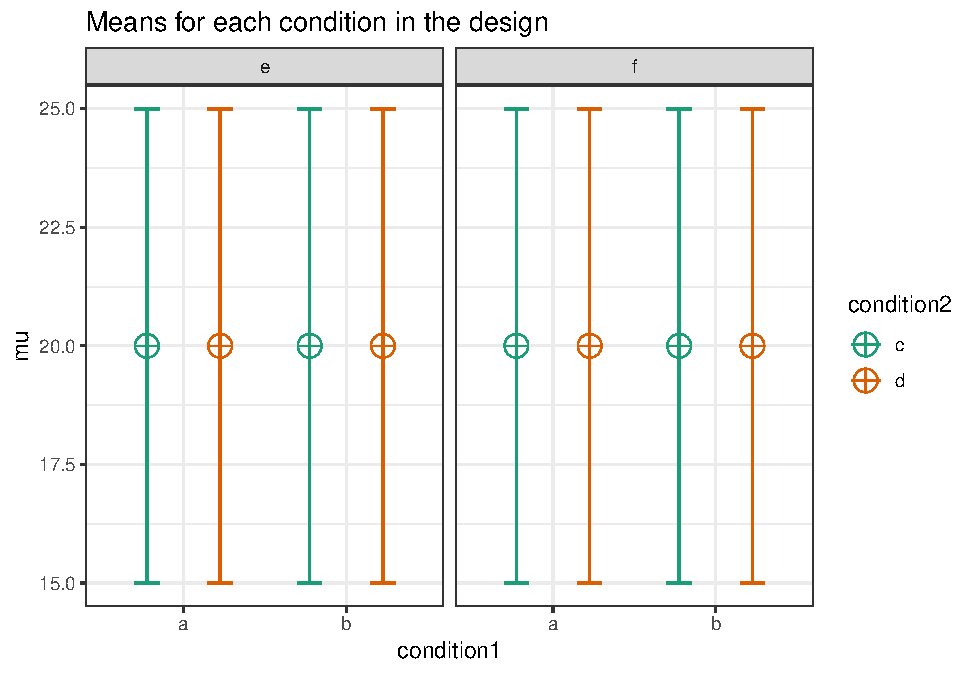
\includegraphics{4.1_error_control_in_exploratory_ANOVA_files/figure-latex/unnamed-chunk-1-1.pdf}

\begin{Shaded}
\begin{Highlighting}[]
\NormalTok{alpha_level <-}\StringTok{ }\FloatTok{0.05}
\CommentTok{#We set the alpha level at 0.05. }

\NormalTok{power_result <-}\StringTok{ }\KeywordTok{ANOVA_power}\NormalTok{(design_result, }\DataTypeTok{alpha_level =}\NormalTok{ alpha_level, }\DataTypeTok{nsims =}\NormalTok{ nsims)}
\end{Highlighting}
\end{Shaded}

\begin{verbatim}
## Power and Effect sizes for ANOVA tests
##                                        power effect size
## anova_condition1                       5.052      0.0012
## anova_condition2                       4.968      0.0012
## anova_condition3                       5.065      0.0012
## anova_condition1:condition2            4.927      0.0011
## anova_condition1:condition3            4.888      0.0012
## anova_condition2:condition3            4.972      0.0012
## anova_condition1:condition2:condition3 5.080      0.0011
## 
## Power and Effect sizes for contrasts
##                                                                                 power effect size
## p_condition1_a_condition2_c_condition3_e_condition1_a_condition2_c_condition3_f 4.936     -0.0001
## p_condition1_a_condition2_c_condition3_e_condition1_a_condition2_d_condition3_e 4.997     -0.0001
## p_condition1_a_condition2_c_condition3_e_condition1_a_condition2_d_condition3_f 4.916     -0.0007
## p_condition1_a_condition2_c_condition3_e_condition1_b_condition2_c_condition3_e 4.880     -0.0003
## p_condition1_a_condition2_c_condition3_e_condition1_b_condition2_c_condition3_f 5.027     -0.0003
## p_condition1_a_condition2_c_condition3_e_condition1_b_condition2_d_condition3_e 5.014     -0.0006
## p_condition1_a_condition2_c_condition3_e_condition1_b_condition2_d_condition3_f 5.034     -0.0006
## p_condition1_a_condition2_c_condition3_f_condition1_a_condition2_d_condition3_e 4.983      0.0000
## p_condition1_a_condition2_c_condition3_f_condition1_a_condition2_d_condition3_f 4.893     -0.0005
## p_condition1_a_condition2_c_condition3_f_condition1_b_condition2_c_condition3_e 4.981     -0.0001
## p_condition1_a_condition2_c_condition3_f_condition1_b_condition2_c_condition3_f 4.924     -0.0002
## p_condition1_a_condition2_c_condition3_f_condition1_b_condition2_d_condition3_e 4.979     -0.0005
## p_condition1_a_condition2_c_condition3_f_condition1_b_condition2_d_condition3_f 4.988     -0.0005
## p_condition1_a_condition2_d_condition3_e_condition1_a_condition2_d_condition3_f 4.845     -0.0005
## p_condition1_a_condition2_d_condition3_e_condition1_b_condition2_c_condition3_e 4.931     -0.0002
## p_condition1_a_condition2_d_condition3_e_condition1_b_condition2_c_condition3_f 5.094     -0.0001
## p_condition1_a_condition2_d_condition3_e_condition1_b_condition2_d_condition3_e 5.026     -0.0005
## p_condition1_a_condition2_d_condition3_e_condition1_b_condition2_d_condition3_f 5.000     -0.0005
## p_condition1_a_condition2_d_condition3_f_condition1_b_condition2_c_condition3_e 5.035      0.0004
## p_condition1_a_condition2_d_condition3_f_condition1_b_condition2_c_condition3_f 4.964      0.0004
## p_condition1_a_condition2_d_condition3_f_condition1_b_condition2_d_condition3_e 4.900      0.0001
## p_condition1_a_condition2_d_condition3_f_condition1_b_condition2_d_condition3_f 4.970      0.0001
## p_condition1_b_condition2_c_condition3_e_condition1_b_condition2_c_condition3_f 4.997      0.0000
## p_condition1_b_condition2_c_condition3_e_condition1_b_condition2_d_condition3_e 4.910     -0.0003
## p_condition1_b_condition2_c_condition3_e_condition1_b_condition2_d_condition3_f 5.067     -0.0003
## p_condition1_b_condition2_c_condition3_f_condition1_b_condition2_d_condition3_e 4.981     -0.0003
## p_condition1_b_condition2_c_condition3_f_condition1_b_condition2_d_condition3_f 4.938     -0.0003
## p_condition1_b_condition2_d_condition3_e_condition1_b_condition2_d_condition3_f 5.100     -0.0001
\end{verbatim}

When there is no true effect, we formally do not have `power' (which is
defined as the probability of finding p \textless{} \(\alpha\) if there
is a true effect to be found) so the power column should be read as the
`Type 1 error rate'. Because we have saved the power simulation in the
`power\_result' object, we can perform calculations on the `sim\_data'
dataframe that is stored. This dataframe contains the results for the
nsims simulations (e.g., 10000 rows if you ran 10000 simulations) and
stores the p-values and effect size estimates for each ANOVA. The first
7 columns are the p-values for the ANOVA, first the main effects of
condition 1, 2, and 3, then three two-way interactions, and finally the
threeway interaction.

We can calculate the number of significant results for each test (which
should be 5\%) by counting the number of significant p-values in each of
the 7 rows:

\begin{Shaded}
\begin{Highlighting}[]
\KeywordTok{apply}\NormalTok{(}\KeywordTok{as.matrix}\NormalTok{(power_result}\OperatorTok{$}\NormalTok{sim_data[(}\DecValTok{1}\OperatorTok{:}\DecValTok{7}\NormalTok{)]), }\DecValTok{2}\NormalTok{, }
    \ControlFlowTok{function}\NormalTok{(x) }\KeywordTok{round}\NormalTok{(}\KeywordTok{mean}\NormalTok{(}\KeywordTok{ifelse}\NormalTok{(x }\OperatorTok{<}\StringTok{ }\NormalTok{alpha_level, }\DecValTok{1}\NormalTok{, }\DecValTok{0}\NormalTok{) }\OperatorTok{*}\StringTok{ }\DecValTok{100}\NormalTok{),}\DecValTok{4}\NormalTok{))}
\end{Highlighting}
\end{Shaded}

\begin{verbatim}
##                       anova_condition1                       anova_condition2                       anova_condition3            anova_condition1:condition2            anova_condition1:condition3 
##                                  5.052                                  4.968                                  5.065                                  4.927                                  4.888 
##            anova_condition2:condition3 anova_condition1:condition2:condition3 
##                                  4.972                                  5.080
\end{verbatim}

This is the Type 1 error rate for each test. When we talk about error
rate inflation due to multiple comparisons, we are talking about the
probability that you conclude there is an effect, when there is actually
no effect, when there is a significant effect for the main effect of
condition 1, or condition 2, or condition 3, or for the two-way
interaction between condition 1 and 2, or condition 1 and 3, or
condition 2 and 3, or in the threeway interaction.

To calculate this error rate we do not just add the 7 error rates (so 7
* 5\% - 35\%). Instead, we calculate the probability that there will be
at least one significant result in an ANOVA we perform. Some ANOVA
results will have multiple significant results, just due to the Type 1
error rate (e.g., a significant result for the threeway interaction, and
for the main effect of condition 1) but such an ANOVA is counted only
once. Iwe calculate this percentage from our simulations, we see the
number is indeed very close to 1-(0.95)\^{}7 = 30\%.

\begin{Shaded}
\begin{Highlighting}[]
\KeywordTok{sum}\NormalTok{(}\KeywordTok{apply}\NormalTok{(}\KeywordTok{as.matrix}\NormalTok{(power_result}\OperatorTok{$}\NormalTok{sim_data[(}\DecValTok{1}\OperatorTok{:}\DecValTok{7}\NormalTok{)]), }\DecValTok{1}\NormalTok{, }
    \ControlFlowTok{function}\NormalTok{(x) }\KeywordTok{round}\NormalTok{(}\KeywordTok{mean}\NormalTok{(}\KeywordTok{ifelse}\NormalTok{(x }\OperatorTok{<}\StringTok{ }\NormalTok{alpha_level, }\DecValTok{1}\NormalTok{, }\DecValTok{0}\NormalTok{) }\OperatorTok{*}\StringTok{ }\DecValTok{100}\NormalTok{),}\DecValTok{4}\NormalTok{)) }\OperatorTok{>}\StringTok{ }\DecValTok{0}\NormalTok{)}\OperatorTok{/}\NormalTok{nsims}\OperatorTok{*}\DecValTok{100}
\end{Highlighting}
\end{Shaded}

\begin{verbatim}
## [1] 29.997
\end{verbatim}

The question is what we should do about this alpha inflation. It is
undesirable if you perform exploratory ANOVA's and are fooled too often
by Type 1 errors, which will not replicate if you try to build on them.
Therefore, you need to control the Type 1 error rate.

In the simulation code, which relies on the afex package, there is the
option to set p\_adjust. In the simulation above, p\_adjust was set to
``none''. This means no adjustment is mage to which p-values are
considered to be significant, and the alpha level is used as it is set
in the simulation (above this was 0.05).

Afex relies on the p.adjust functon in the stats package in R (more
information is available
\href{https://www.rdocumentation.org/packages/stats/versions/3.1.1/topics/p.adjust}{here}).
From the package details:

\emph{The adjustment methods include the Bonferroni correction
(``bonferroni'') in which the p-values are multiplied by the number of
comparisons. Less conservative corrections are also included by Holm
(1979) (``holm''), Hochberg (1988) (``hochberg''), Hommel (1988)
(``hommel''), Benjamini \& Hochberg (1995) (``BH'' or its alias
``fdr''), and Benjamini \& Yekutieli (2001) (``BY''), respectively. A
pass-through option (``none'') is also included. The first four methods
are designed to give strong control of the family-wise error rate. There
seems no reason to use the unmodified Bonferroni correction because it
is dominated by Holm's method, which is also valid under arbitrary
assumptions.}

\emph{Hochberg's and Hommel's methods are valid when the hypothesis
tests are independent or when they are non-negatively associated
(Sarkar, 1998; Sarkar and Chang, 1997). Hommel's method is more powerful
than Hochberg's, but the difference is usually small and the Hochberg
p-values are faster to compute.}

\emph{The ``BH'' (aka ``fdr'') and ``BY'' method of Benjamini, Hochberg,
and Yekutieli control the false discovery rate, the expected proportion
of false discoveries amongst the rejected hypotheses. The false
discovery rate is a less stringent condition than the family-wise error
rate, so these methods are more powerful than the others.}

Let's re-run the simulation twith the Holm-Bonferroni correction, which
is simple and require no assumptions.

\begin{Shaded}
\begin{Highlighting}[]
\NormalTok{string <-}\StringTok{ "2b*2b*2b"}
\NormalTok{n <-}\StringTok{ }\DecValTok{50}
\NormalTok{mu <-}\StringTok{ }\KeywordTok{c}\NormalTok{(}\DecValTok{20}\NormalTok{, }\DecValTok{20}\NormalTok{, }\DecValTok{20}\NormalTok{, }\DecValTok{20}\NormalTok{, }\DecValTok{20}\NormalTok{, }\DecValTok{20}\NormalTok{, }\DecValTok{20}\NormalTok{, }\DecValTok{20}\NormalTok{) }\CommentTok{#All means are equal - so there is no real difference.}
\CommentTok{# Enter means in the order that matches the labels below.}
\NormalTok{sd <-}\StringTok{ }\DecValTok{5}
\NormalTok{r <-}\StringTok{ }\DecValTok{0} 
\CommentTok{# (note that since we simulate a between design, the correlation between variables }
\CommentTok{# will be 0, regardless of what you enter here, but the value must be set).}
\NormalTok{p_adjust =}\StringTok{ "holm"}
\CommentTok{# Changed to Holm-Bonferroni}
\NormalTok{labelnames <-}\StringTok{ }\KeywordTok{c}\NormalTok{(}\StringTok{"condition1"}\NormalTok{, }\StringTok{"a"}\NormalTok{, }\StringTok{"b"}\NormalTok{, }\StringTok{"condition2"}\NormalTok{, }\StringTok{"c"}\NormalTok{, }\StringTok{"d"}\NormalTok{, }\StringTok{"condition3"}\NormalTok{, }\StringTok{"e"}\NormalTok{, }\StringTok{"f"}\NormalTok{) }\CommentTok{#}
\CommentTok{# the label names should be in the order of the means specified above.}

\NormalTok{design_result <-}\StringTok{ }\KeywordTok{ANOVA_design}\NormalTok{(}\DataTypeTok{string =}\NormalTok{ string,}
                   \DataTypeTok{n =}\NormalTok{ n, }
                   \DataTypeTok{mu =}\NormalTok{ mu, }
                   \DataTypeTok{sd =}\NormalTok{ sd, }
                   \DataTypeTok{r =}\NormalTok{ r, }
                   \DataTypeTok{p_adjust =}\NormalTok{ p_adjust,}
                   \DataTypeTok{labelnames =}\NormalTok{ labelnames)}
\end{Highlighting}
\end{Shaded}

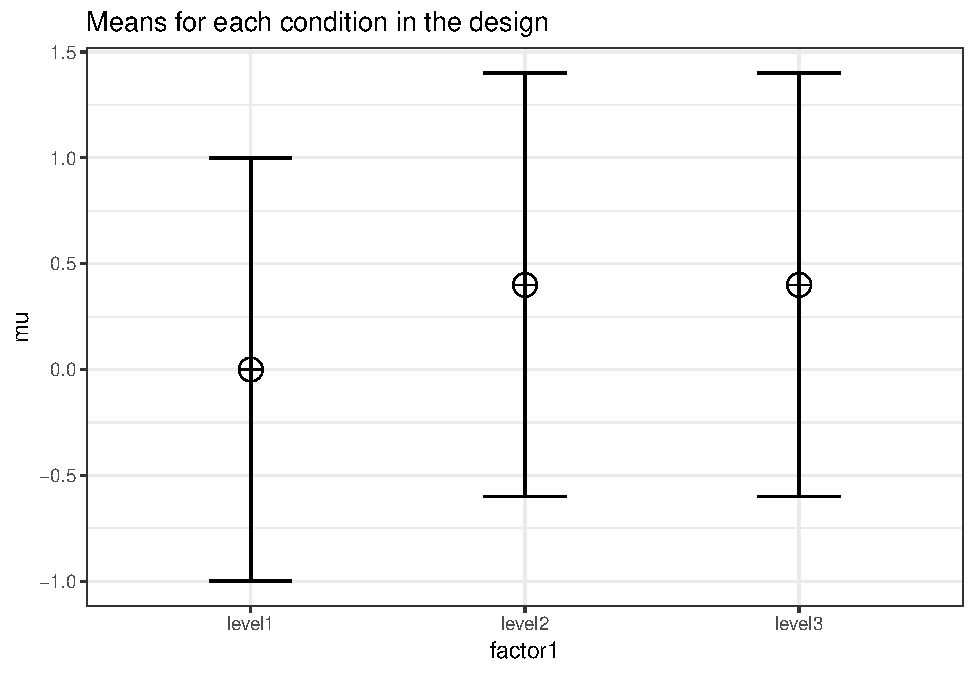
\includegraphics{4.1_error_control_in_exploratory_ANOVA_files/figure-latex/unnamed-chunk-4-1.pdf}

\begin{Shaded}
\begin{Highlighting}[]
\NormalTok{alpha_level <-}\StringTok{ }\FloatTok{0.05}
\CommentTok{#We set the alpha level at 0.05. }

\NormalTok{power_result <-}\StringTok{ }\KeywordTok{ANOVA_power}\NormalTok{(design_result, }\DataTypeTok{alpha_level =}\NormalTok{ alpha_level, }\DataTypeTok{nsims =}\NormalTok{ nsims)}
\end{Highlighting}
\end{Shaded}

\begin{verbatim}
## Power and Effect sizes for ANOVA tests
##                                        power effect size
## anova_condition1                       0.785      0.0011
## anova_condition2                       0.721      0.0011
## anova_condition3                       0.696      0.0012
## anova_condition1:condition2            0.770      0.0012
## anova_condition1:condition3            0.752      0.0012
## anova_condition2:condition3            0.707      0.0012
## anova_condition1:condition2:condition3 0.726      0.0012
## 
## Power and Effect sizes for contrasts
##                                                                                 power effect size
## p_condition1_a_condition2_c_condition3_e_condition1_a_condition2_c_condition3_f 4.944     -0.0002
## p_condition1_a_condition2_c_condition3_e_condition1_a_condition2_d_condition3_e 5.026      0.0000
## p_condition1_a_condition2_c_condition3_e_condition1_a_condition2_d_condition3_f 5.039     -0.0005
## p_condition1_a_condition2_c_condition3_e_condition1_b_condition2_c_condition3_e 5.003      0.0014
## p_condition1_a_condition2_c_condition3_e_condition1_b_condition2_c_condition3_f 5.035      0.0000
## p_condition1_a_condition2_c_condition3_e_condition1_b_condition2_d_condition3_e 4.922      0.0005
## p_condition1_a_condition2_c_condition3_e_condition1_b_condition2_d_condition3_f 4.953     -0.0005
## p_condition1_a_condition2_c_condition3_f_condition1_a_condition2_d_condition3_e 5.127      0.0003
## p_condition1_a_condition2_c_condition3_f_condition1_a_condition2_d_condition3_f 4.976     -0.0003
## p_condition1_a_condition2_c_condition3_f_condition1_b_condition2_c_condition3_e 5.059      0.0016
## p_condition1_a_condition2_c_condition3_f_condition1_b_condition2_c_condition3_f 5.166      0.0004
## p_condition1_a_condition2_c_condition3_f_condition1_b_condition2_d_condition3_e 5.024      0.0008
## p_condition1_a_condition2_c_condition3_f_condition1_b_condition2_d_condition3_f 4.872     -0.0002
## p_condition1_a_condition2_d_condition3_e_condition1_a_condition2_d_condition3_f 5.198     -0.0006
## p_condition1_a_condition2_d_condition3_e_condition1_b_condition2_c_condition3_e 5.050      0.0013
## p_condition1_a_condition2_d_condition3_e_condition1_b_condition2_c_condition3_f 5.075      0.0000
## p_condition1_a_condition2_d_condition3_e_condition1_b_condition2_d_condition3_e 5.129      0.0004
## p_condition1_a_condition2_d_condition3_e_condition1_b_condition2_d_condition3_f 5.044     -0.0005
## p_condition1_a_condition2_d_condition3_f_condition1_b_condition2_c_condition3_e 4.931      0.0019
## p_condition1_a_condition2_d_condition3_f_condition1_b_condition2_c_condition3_f 5.058      0.0006
## p_condition1_a_condition2_d_condition3_f_condition1_b_condition2_d_condition3_e 5.049      0.0011
## p_condition1_a_condition2_d_condition3_f_condition1_b_condition2_d_condition3_f 4.989      0.0001
## p_condition1_b_condition2_c_condition3_e_condition1_b_condition2_c_condition3_f 5.039     -0.0012
## p_condition1_b_condition2_c_condition3_e_condition1_b_condition2_d_condition3_e 5.079     -0.0009
## p_condition1_b_condition2_c_condition3_e_condition1_b_condition2_d_condition3_f 4.939     -0.0018
## p_condition1_b_condition2_c_condition3_f_condition1_b_condition2_d_condition3_e 5.007      0.0004
## p_condition1_b_condition2_c_condition3_f_condition1_b_condition2_d_condition3_f 4.918     -0.0005
## p_condition1_b_condition2_d_condition3_e_condition1_b_condition2_d_condition3_f 4.981     -0.0010
\end{verbatim}

If we now calculate the overall Type 1 error rate:

\begin{Shaded}
\begin{Highlighting}[]
\KeywordTok{sum}\NormalTok{(}\KeywordTok{apply}\NormalTok{(}\KeywordTok{as.matrix}\NormalTok{(power_result}\OperatorTok{$}\NormalTok{sim_data[(}\DecValTok{1}\OperatorTok{:}\DecValTok{7}\NormalTok{)]), }\DecValTok{1}\NormalTok{, }
    \ControlFlowTok{function}\NormalTok{(x) }\KeywordTok{round}\NormalTok{(}\KeywordTok{mean}\NormalTok{(}\KeywordTok{ifelse}\NormalTok{(x }\OperatorTok{<}\StringTok{ }\NormalTok{alpha_level, }\DecValTok{1}\NormalTok{, }\DecValTok{0}\NormalTok{) }\OperatorTok{*}\StringTok{ }\DecValTok{100}\NormalTok{),}\DecValTok{4}\NormalTok{)) }\OperatorTok{>}\StringTok{ }\DecValTok{0}\NormalTok{)}\OperatorTok{/}\NormalTok{nsims}\OperatorTok{*}\DecValTok{100}
\end{Highlighting}
\end{Shaded}

\begin{verbatim}
## [1] 4.991
\end{verbatim}

We see it is close to 5\%. Note that error rates have variation, and
even in a few thousand simulations, the error rate in the sample of
studies can easily be half a percentage point higher or lower. But
\emph{in the long run} the error rate should equal the alpha level.
Furthermore, note that the
\href{https://en.wikipedia.org/wiki/Holm\%E2\%80\%93Bonferroni_method}{Holm-bonferroni}
method is slightly more powerful than the Bonferroni procedure (which is
simply \(\alpha\) divided by the numner of tests). There are more
powerful procedures to control the Type 1 error rate, which require more
assumptions. For a small number of tests, they Holm-Bonferroni procedure
works well. Alternative procedure to control error rates can be found in
the
\href{https://cran.r-project.org/web/packages/multcomp/index.html}{multcomp}
R package.


\end{document}
